\begin{figure*}
  \def\tracecsv{figures/data/exp_counting/traces_and_fits.csv}
  \def\histogramcsv{figures/data/exp_counting/intensity_histograms.csv}

  \centerline{
    \def\traceintensitycol{N4_trace_good}
    \def\histbincol{N4_good_bins}
    \def\histcountcol{N4_good_measured}
    \def\modelfitcol{N4_good_model}
    \def\zcol{N4_fit_good}
    \tikzsetnextfilename{figure_5_trace_N4_good}
    \begin{tikzpicture}%
  \begin{axis}[
    name=trace,
    width=0.8\textwidth,
    height=5cm,
    xlabel=frames,
    ylabel=intensity,
    enlarge x limits=false,
    xtick distance=500,
    grid=major,
    grid style={dashed},
    scaled ticks=false,
    ticklabel style={font=\small},
    legend style={nodes={scale=0.6, transform shape}},
  ]

    \addplot [
      color=tracecolor,
      mark=*,
      mark size=0.7pt,
      mark options={line width=0},
      fill opacity=0.8,
      draw opacity=0.2,
    ] table [
      col sep=comma,
      x=frames,
      y=\traceintensitycol
    ] {\tracecsv};
    \addlegendentry{intensity trace}

    \addplot [
      color=ztracecolor,
      thick
    ] table [
      col sep=comma,
      x=frames,
      y=\zcol
    ] {\tracecsv};
    \addlegendentry{inferred state}

    % remember min/max y-axis values for next plot
    \pgfplotsextra{
      \pgfmathparse{\pgfkeysvalueof{/pgfplots/ymin}}
      \global\let\ymin\pgfmathresult
      \pgfmathparse{\pgfkeysvalueof{/pgfplots/ymax}}
      \global\let\ymax\pgfmathresult
    }

  \end{axis}

  \begin{axis}[
    at={($(trace.east) + (4mm,0)$)},
    anchor=west,
    width=0.3\textwidth,
    height=5cm,
    yticklabel=\empty,
    xtick distance=0.005,
    xlabel=probability,
    grid=major,
    grid style={dashed, very thin},
    enlarge x limits={value=0.1,upper},
    scaled ticks=false,
    ymin=\ymin,
    ymax=\ymax,
    ticklabel style={font=\small},
    legend style={nodes={scale=0.6, transform shape}},
  ]

    \addplot+[
      xbar interval,
      mark=none,
      color=tracecolor,
      fill=tracecolor,
      fill opacity=0.6,
      draw=none,
    ] table [
      col sep=comma,
      y=\histbincol,
      x=\histcountcol,
    ] {\histogramcsv};
    \addlegendentry{intensity histogram}

    \addplot[
      color=intensitymodelcolor!80!black,
      thick
    ] table [
      col sep=comma,
      y=\histbincol,
      x=\modelfitcol
    ] {\histogramcsv};
    \addlegendentry{inferred model}

  \end{axis}
\end{tikzpicture}%

  }

  \centerline{
    \def\traceintensitycol{N1_trace_good}
    \def\histbincol{N1_good_bins}
    \def\histcountcol{N1_good_measured}
    \def\modelfitcol{N1_good_model}
    \def\zcol{N1_fit_good}
    \tikzsetnextfilename{figure_5_trace_N1_good}
    \begin{tikzpicture}%
  \begin{axis}[
    name=trace,
    width=0.8\textwidth,
    height=5cm,
    xlabel=frames,
    ylabel=intensity,
    enlarge x limits=false,
    xtick distance=500,
    grid=major,
    grid style={dashed},
    scaled ticks=false,
    ticklabel style={font=\small},
    legend style={nodes={scale=0.6, transform shape}},
  ]

    \addplot [
      color=tracecolor,
      mark=*,
      mark size=0.7pt,
      mark options={line width=0},
      fill opacity=0.8,
      draw opacity=0.2,
    ] table [
      col sep=comma,
      x=frames,
      y=\traceintensitycol
    ] {\tracecsv};
    \addlegendentry{intensity trace}

    \addplot [
      color=ztracecolor,
      thick
    ] table [
      col sep=comma,
      x=frames,
      y=\zcol
    ] {\tracecsv};
    \addlegendentry{inferred state}

    % remember min/max y-axis values for next plot
    \pgfplotsextra{
      \pgfmathparse{\pgfkeysvalueof{/pgfplots/ymin}}
      \global\let\ymin\pgfmathresult
      \pgfmathparse{\pgfkeysvalueof{/pgfplots/ymax}}
      \global\let\ymax\pgfmathresult
    }

  \end{axis}

  \begin{axis}[
    at={($(trace.east) + (4mm,0)$)},
    anchor=west,
    width=0.3\textwidth,
    height=5cm,
    yticklabel=\empty,
    xtick distance=0.005,
    xlabel=probability,
    grid=major,
    grid style={dashed, very thin},
    enlarge x limits={value=0.1,upper},
    scaled ticks=false,
    ymin=\ymin,
    ymax=\ymax,
    ticklabel style={font=\small},
    legend style={nodes={scale=0.6, transform shape}},
  ]

    \addplot+[
      xbar interval,
      mark=none,
      color=tracecolor,
      fill=tracecolor,
      fill opacity=0.6,
      draw=none,
    ] table [
      col sep=comma,
      y=\histbincol,
      x=\histcountcol,
    ] {\histogramcsv};
    \addlegendentry{intensity histogram}

    \addplot[
      color=intensitymodelcolor!80!black,
      thick
    ] table [
      col sep=comma,
      y=\histbincol,
      x=\modelfitcol
    ] {\histogramcsv};
    \addlegendentry{inferred model}

  \end{axis}
\end{tikzpicture}%

  }
\end{figure*}


\begin{figure*}
  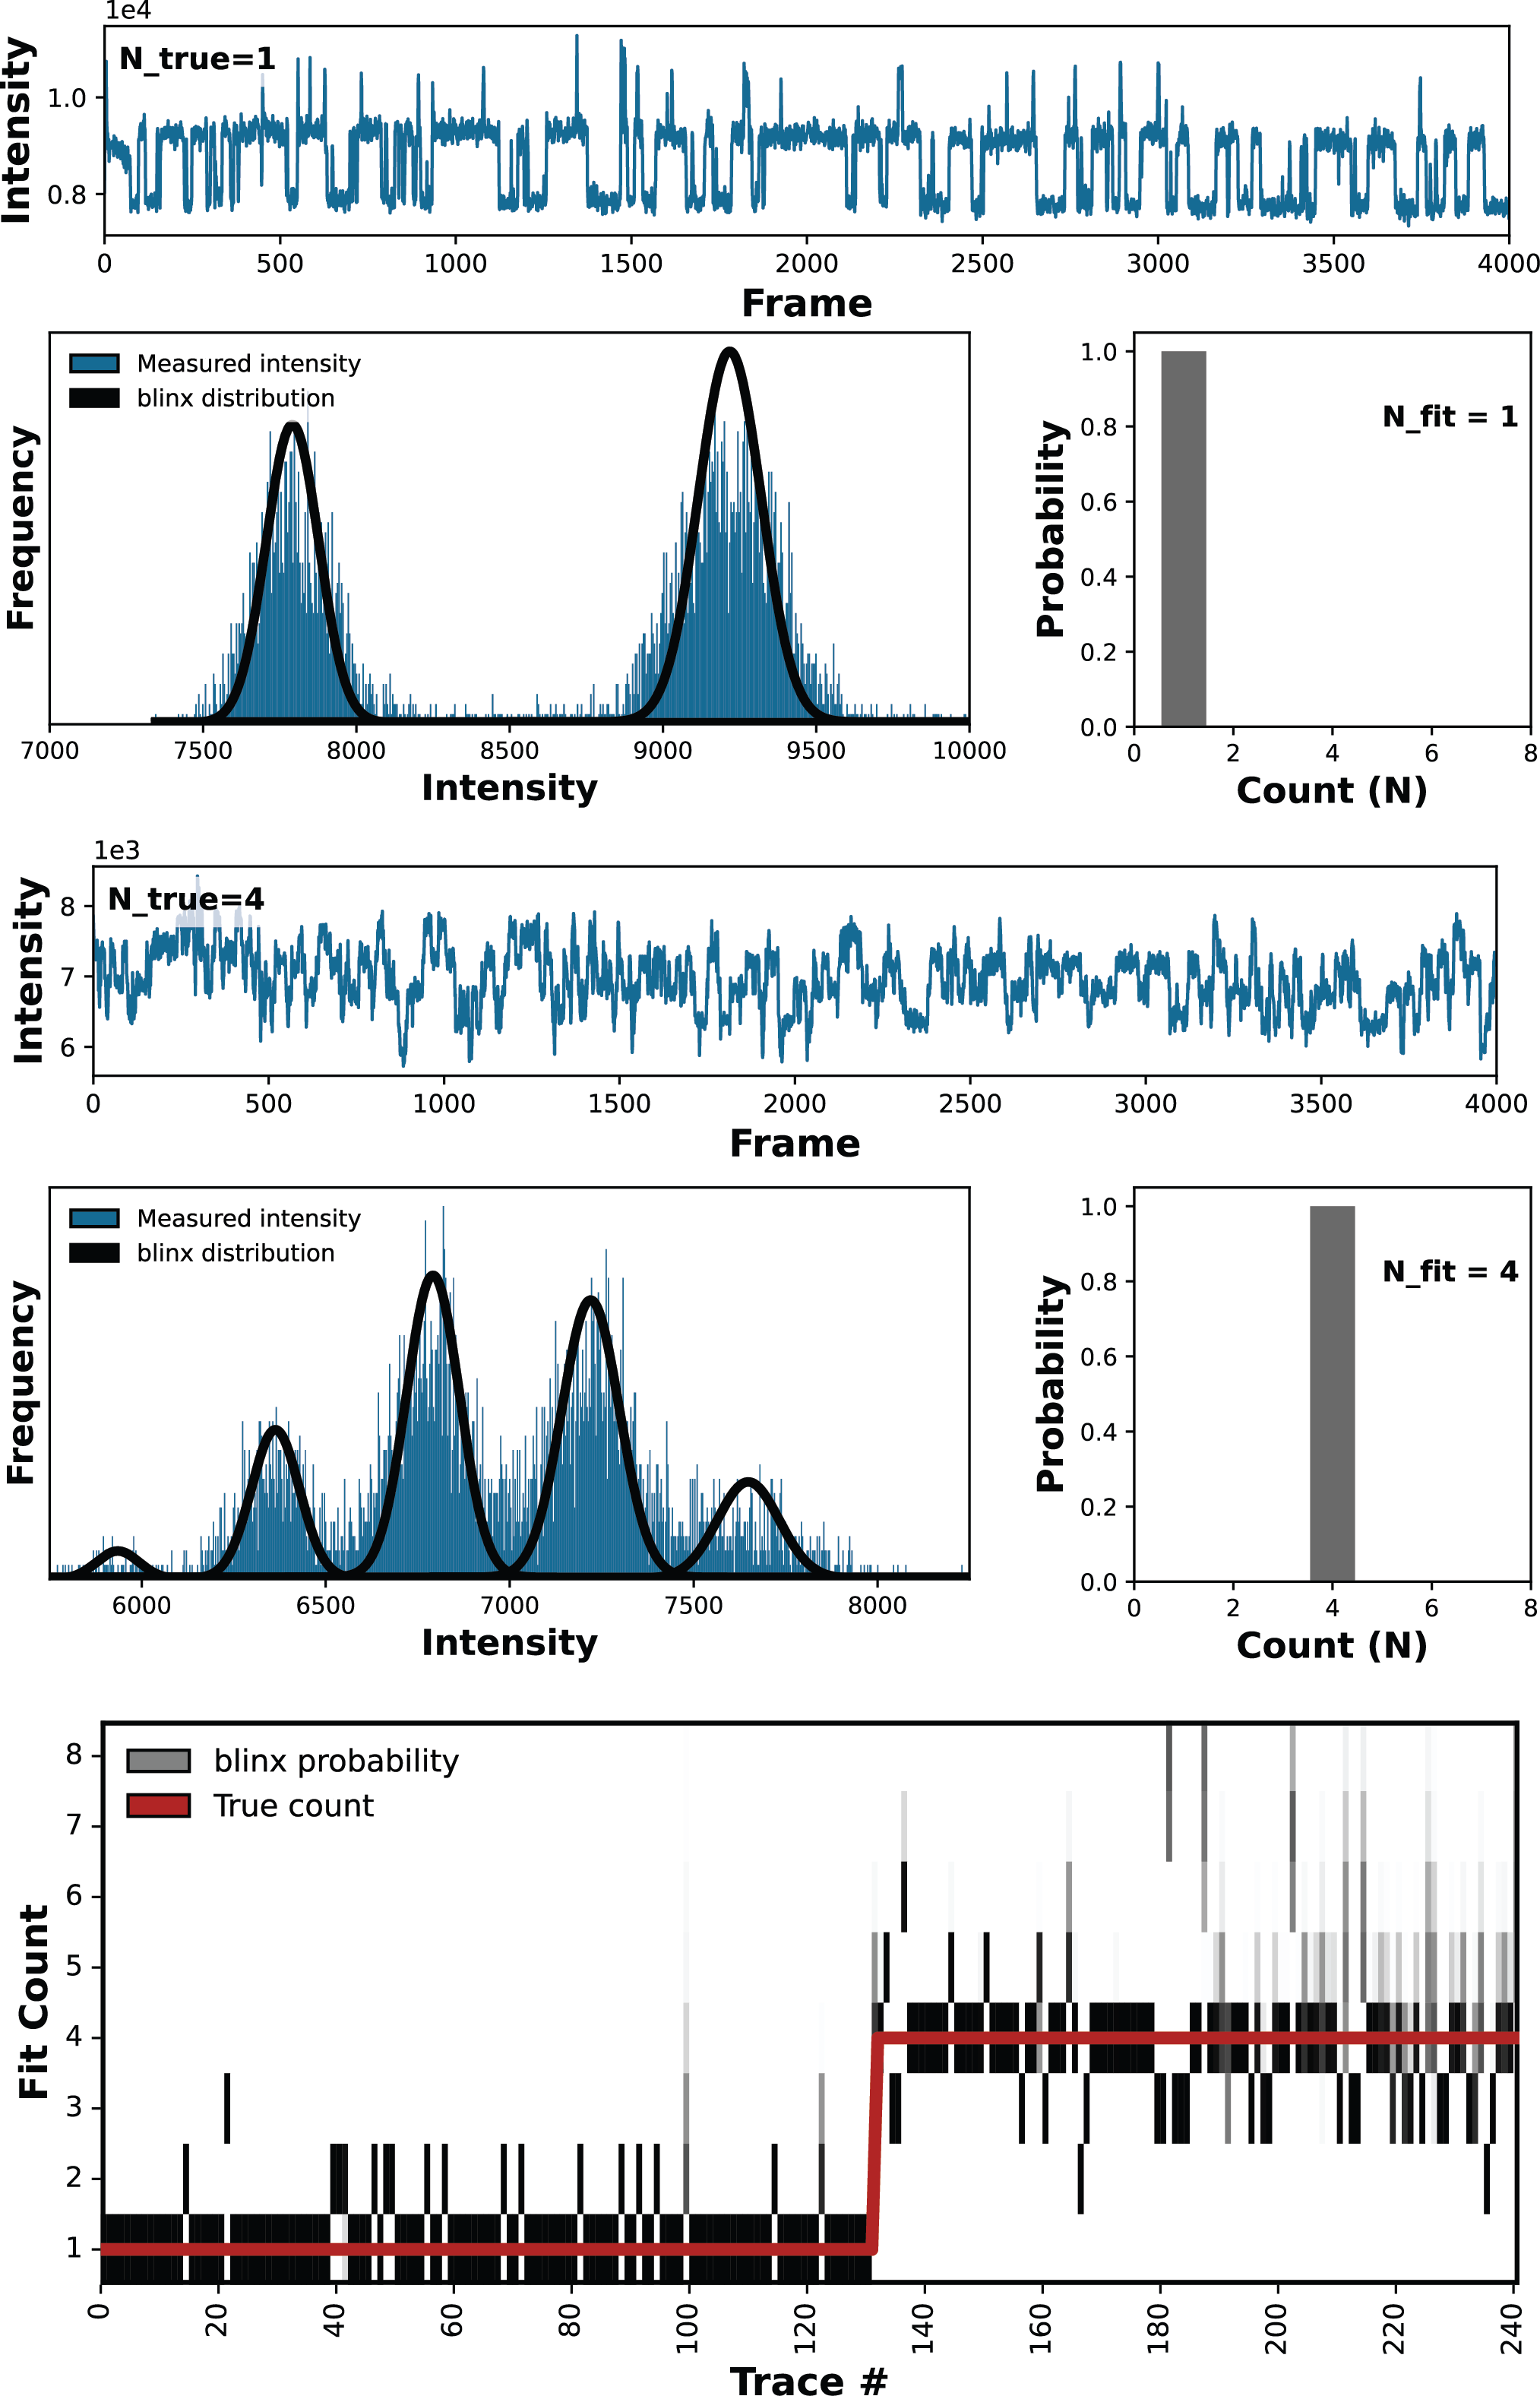
\includegraphics[width=\linewidth]{figures/placeholders/figure_5_experimental_counting.png}
  \caption{experimental counting}
  \label{fig:method:overview}
\end{figure*}
